\documentclass[../AnalysisNoteJBuxton.tex]{subfiles}
\begin{document}

\subsection{Model: Lambda-Kaon}
\label{ModelLambdaKaon}

In the absence of Coulomb effects, and assuming a spherically gaussian source of width $R$, the 1D femtoscopic correlation function can be calculated analytically using:

\begin{equation}
 C(k^{*}) = 1 + \lambda[C_{QI}(k^{*}) + C_{FSI}(k^{*})]
\label{eqn:LednickyEqn}
\end{equation}

$C_{QI}$ describes plane-wave quantum interference:

\begin{equation}
 C_{QI}(k^{*}) = \alpha\exp(-4k^{*2}R^{2})
\label{eqn:CQI}
\end{equation}

where $\alpha = (-1)^{2j}/(2j+1)$ for identical particles with spin j, and $\alpha = 0$ for non-identical particles.  $C_{FSI}$ describes the s-wave strong final state interaction between the particles:

\begin{equation}
\begin{array}{l}
\vspace{2mm}  %%space between C_{FSI}(k^{*}) and f(k^{*})
  C_{FSI}(k^{*}) = (1+\alpha)[\frac{1}{2}|\frac{f(k^{*})}{R}|^2(1-\frac{d_{0}}{2\sqrt{\pi}R})+\frac{2\mathbb{R}f(k^{*})}{\sqrt{\pi}R}F_{1}(2k^{*}R)-\frac{\mathbb{I}f(k^{*})}{R}F_{2}(2k^{*}R)] \\
\vspace{2mm}  %%space after f(k^{*})  
  ~~~~~f(k^{*}) = (\frac{1}{f_{0}}+\frac{1}{2}d_{0}k^{*2}-ik^{*})^{-1};~~~
  F_{1}(z) = \int_{0}^{z} \frac{e^{x^{2}-z^{2}}}{z}dx;~~~
  F_{2}(z) = \frac{1-e^{-z^{2}}}{z}
\end{array}  
\label{eqn:CFSI}
\end{equation}

where $R$ is the source size, $f(k^{*})$ is the s-wave scattering amplitude, $f_{0}$ is the complex scattering length, and $d_{0}$ is the effective range of the interaction.

The code developed to fit the data is called ``LednickyFitter", and utilizes the ROOT TMinuit implementation of the MINUIT fitting package.
In short, given a function with a number of parameters, the fitter explores the parameter space searching for the minimum of the equation.
In this implementation, the function to be minimized should represent the difference between the measure and theoretical correlation functions.
However, a simple $\chi^{2}$ test in inappropriate for fitting correlation functions, as the ratio two Poisson distributions does not result in a Poisson distribution.
Instead, a log-likelihood fit function of the following form is used \cite{Lisa:2005dd}:

\begin{equation}
 \chi^{2}_{PML} = -2\left[A\ln\left(\frac{C(A+B)}{A(C+1)}\right) + B\ln\left(\frac{A+B}{B(C+1)}\right)\right]
\label{eqn:Chi2PML}
\end{equation}

where $A$ is the experimental signal distribution (numerator), $B$ is the experimental background distribution (denominator), and $C$ is the theoretical fit correlation function.

The LednickyFitter uses Equations \ref{eqn:LednickyEqn} -- \ref{eqn:CFSI} to build the theoretical fit, and Equation \ref{eqn:Chi2PML} as the statistic quantifying the quality of the fit.
The parameters to be varied by MINUIT are: $\lambda$, $R$, $f_{0}$ ($\mathbb{R}f_{0}$ and $\mathbb{I}f_{0}$ separately), $d_{0}$, and normalization $N$.
The fitter currently includes methods to correct for momentum resolution and a non-flat background.
These corrections are applied to the fit function, the data is never touched.
The fitter is able to share parameters between different analyses and fit all simultaneously.  

In a typical fit, a given pair is fit with its conjugate (ex. $\Lambda$K$^{+}$ with $\bar{\Lambda}$K$^{-}$) across all centralities (0-10\%, 10-30\%, 30-50\%), for a total of 6 simultaneous analyses.
Each analysis has a unique $\lambda$ and normalization parameter.
The radii are shared between analyses of like centrality, as these should have similar source sizes.
The scattering parameters ($\mathbb{R}f_{0}$, $\mathbb{I}f_{0}$, $d_{0}$) are shared amongst all.

Figures \ref{fig:LamK0wConjFits}, \ref{fig:LamKchPwConjFits}, and \ref{fig:LamKchMwConjFits} show experimental data with fits for all studied centralities for $\Lambda$K$^{0}_{S}$ with $\bar{\Lambda}$K$^{0}_{S}$, $\Lambda$K$^{+}$ with $\bar{\Lambda}$K$^{-}$, and $\Lambda$K$^{-}$ with $\bar{\Lambda}$K$^{+}$, respectively.  In the figures, the black solid line represents the ``raw" fit, i.e. not corrected for momentum resolution effects nor non-flat background.  The green line shows the fit to the non-flat background.  The purple points show the fit after momentum resolution and non-flat background corrections have been applied.  The initial values of the parameters is listed, as well as the final fit values with uncertainties.

\begin{figure}[h]
  \centering
  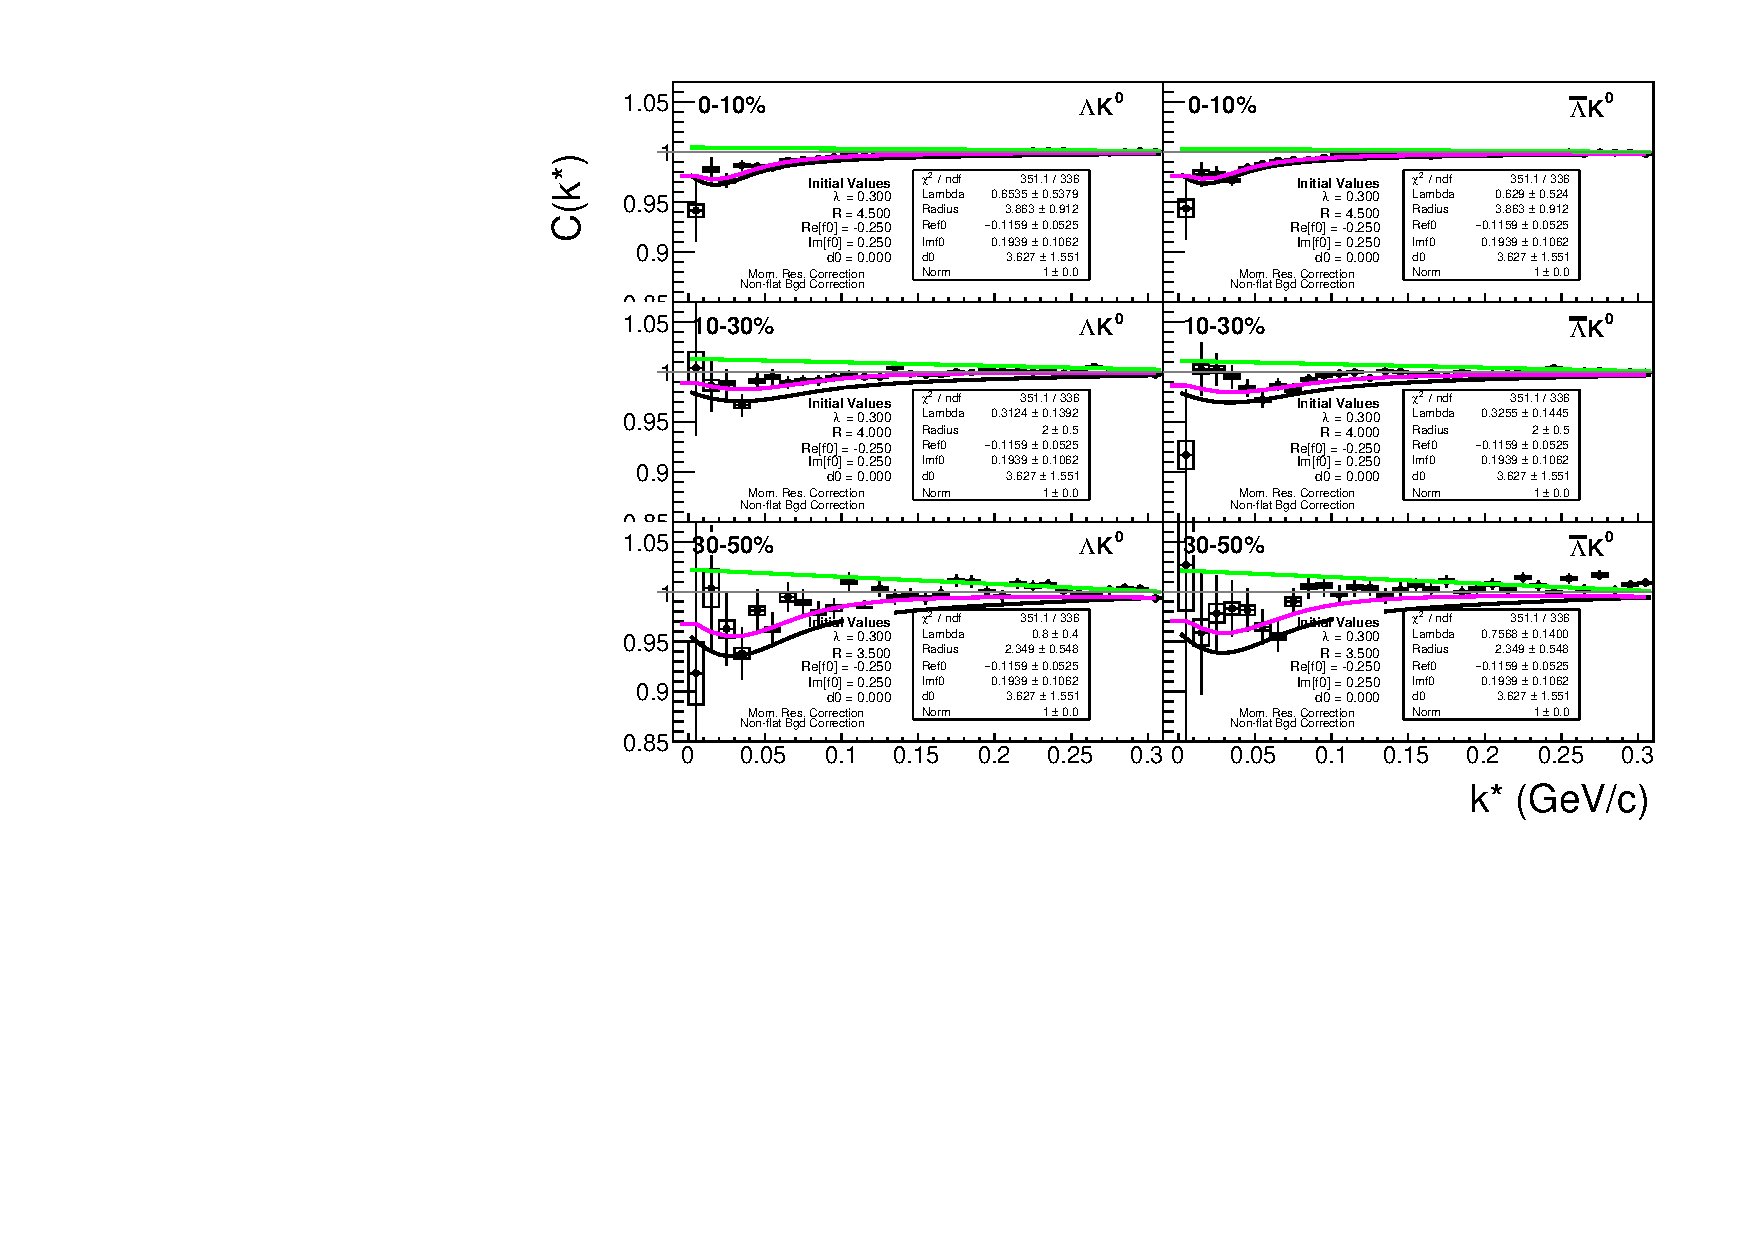
\includegraphics[width=\textwidth]{5_Fitting/Figures/canKStarCfwFitsLamK0wConj_MomResCrctn_NonFlatBgdCrctn.pdf}
  \caption[$\Lambda$K$^{0}_{S}$($\bar{\Lambda}$K$^{0}_{S}$) Fits]{Fits to the $\Lambda$K$^{0}_{S}$ (left) and $\bar{\Lambda}$K$^{0}_{S}$ (right) data for the centralities 0-10\% (top), 10-30\% (middle), and 30-50\% (bottom).
Each has unique $\lambda$ and normalization parameters.
The radii are shared amongst like centralities; the scattering parameters ($\mathbb{R}f_{0}$, $\mathbb{I}f_{0}$, $d_{0}$) are shared amongst all.
The black solid line represents the ``raw" fit, i.e. not corrected for momentum resolution effects nor non-flat background.  
The green line shows the fit to the non-flat background.
The purple points show the fit after momentum resolution and non-flat background corrections have been applied.
The initial values of the parameters is listed, as well as the final fit values with uncertainties.}
  \label{fig:LamK0wConjFits}
\end{figure}


\begin{figure}[h]
  \centering
  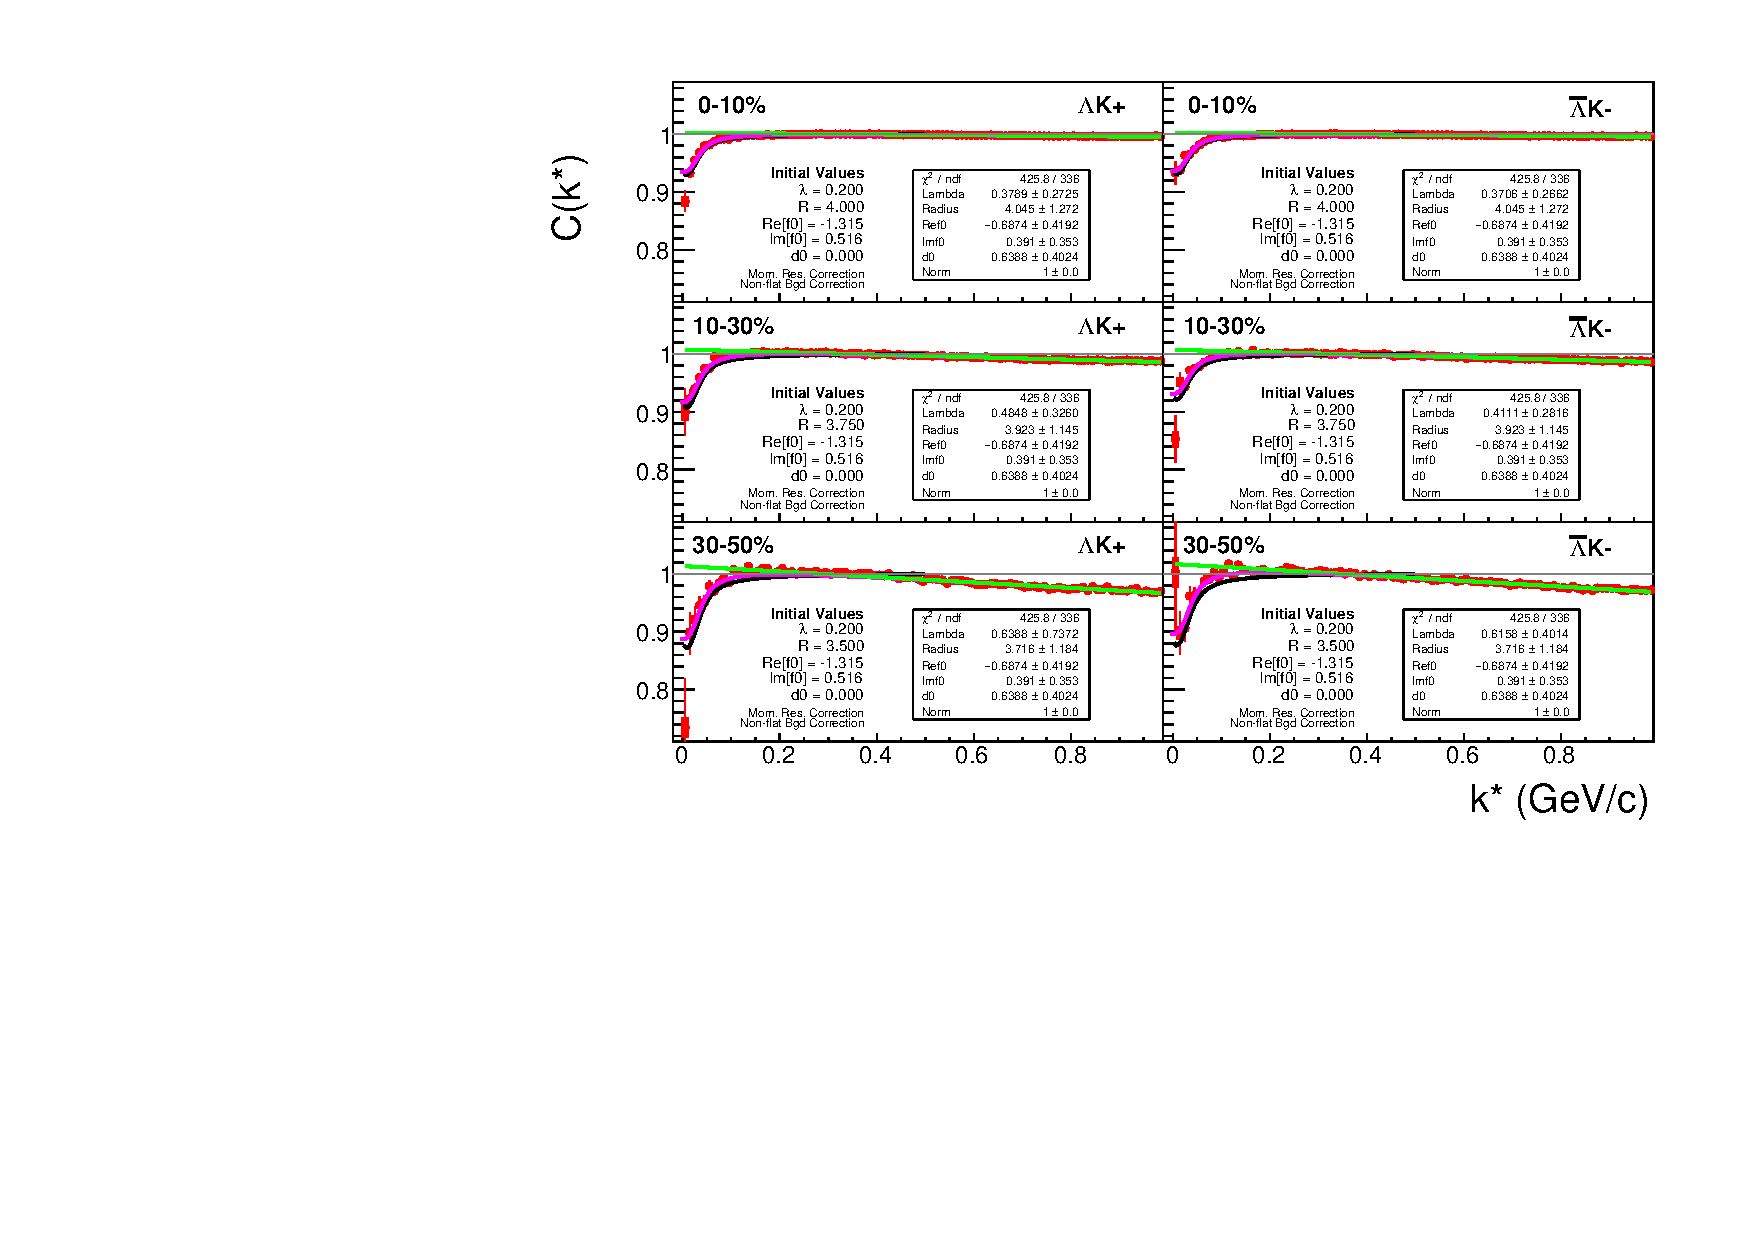
\includegraphics[width=\textwidth]{5_Fitting/Figures/canKStarCfwFitsLamKchPwConj_MomResCrctn_NonFlatBgdCrctn.pdf}
  \caption[$\Lambda$K$^{+}$($\bar{\Lambda}$K$^{-}$) Fits]{Fits to the $\Lambda$K$^{+}$ (left) and $\bar{\Lambda}$K$^{-}$ (right) data for the centralities 0-10\% (top), 10-30\% (middle), and 30-50\% (bottom).
Each has unique $\lambda$ and normalization parameters.
The radii are shared amongst like centralities; the scattering parameters ($\mathbb{R}f_{0}$, $\mathbb{I}f_{0}$, $d_{0}$) are shared amongst all.
The black solid line represents the ``raw" fit, i.e. not corrected for momentum resolution effects nor non-flat background.  
The green line shows the fit to the non-flat background.
The purple points show the fit after momentum resolution and non-flat background corrections have been applied.
The initial values of the parameters is listed, as well as the final fit values with uncertainties.}
  \label{fig:LamKchPwConjFits}
\end{figure}

\begin{figure}[h]
  \centering
  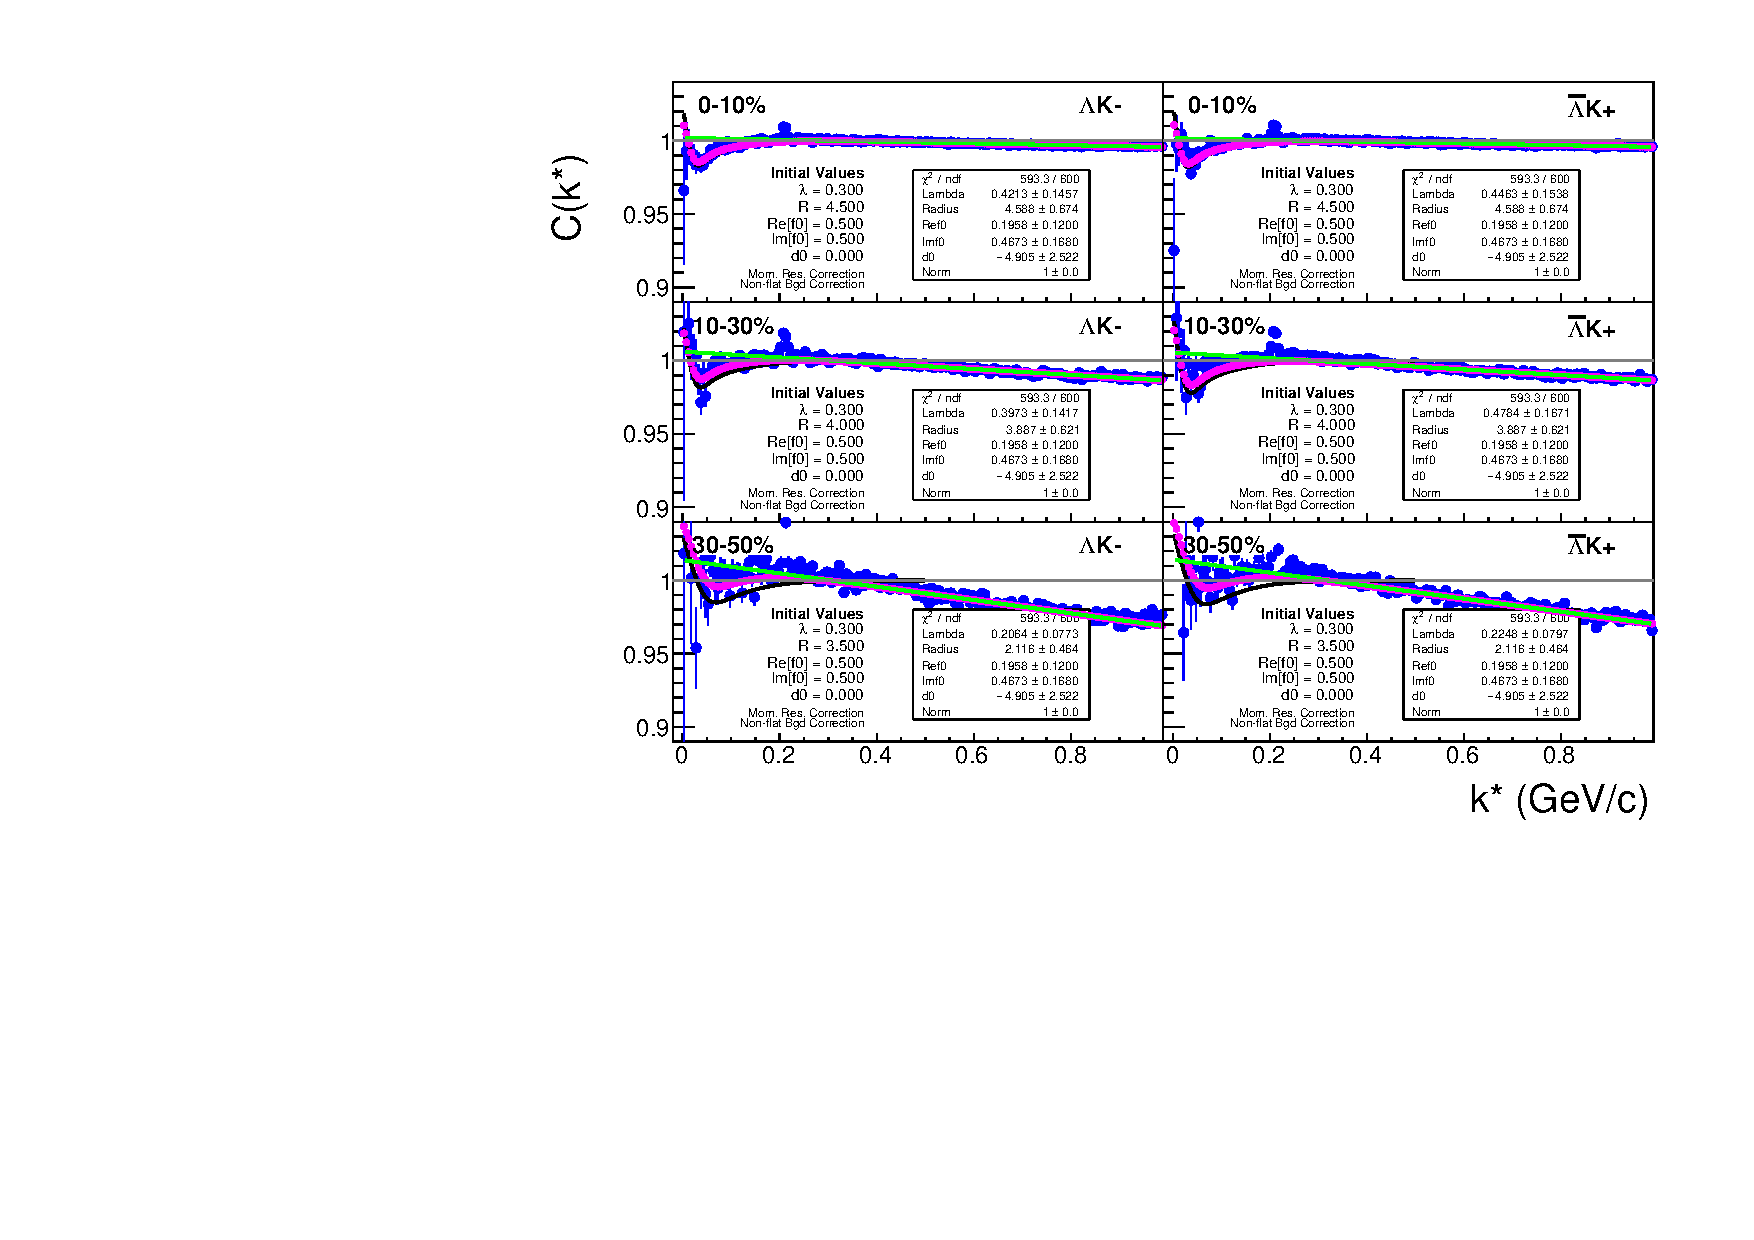
\includegraphics[width=\textwidth]{5_Fitting/Figures/canKStarCfwFitsLamKchMwConj_MomResCrctn_NonFlatBgdCrctn.pdf}
  \caption[$\Lambda$K$^{-}$($\bar{\Lambda}$K$^{+}$) Fits]{Fits to the $\Lambda$K$^{-}$(left) with $\bar{\Lambda}$K$^{+}$ (right) data for the centralities 0-10\% (top), 10-30\% (middle), and 30-50\% (bottom).
Each has unique $\lambda$ and normalization parameters.
The radii are shared amongst like centralities; the scattering parameters ($\mathbb{R}f_{0}$, $\mathbb{I}f_{0}$, $d_{0}$) are shared amongst all.
The black solid line represents the ``raw" fit, i.e. not corrected for momentum resolution effects nor non-flat background.  
The green line shows the fit to the non-flat background.
The purple points show the fit after momentum resolution and non-flat background corrections have been applied.
The initial values of the parameters is listed, as well as the final fit values with uncertainties.}
  \label{fig:LamKchMwConjFits}
\end{figure}

\end{document}